\section{Auswertung}
\label{sec:Auswertung}
Aufgrund der zahlreichen Messwerte kann man die zeitlichen Temperaturverläufe sehr genau darstellen.
In den beiden folgenden Abbildungen sind die Temperaturen der äußeren Sensoren von 
Messing(breit)[T1], Messing(schmal)[T4] sowie Aluminium[T5] und Edelstahl[T8] gegenübergestellt, die bei der 
statischen Methode aufgenommen worden sind.
% side-by-side Gegenüberstellung der ersten beiden plots
\begin{figure}
    \centering
    \begin{subfigure}{.5\textwidth}
        \centering
        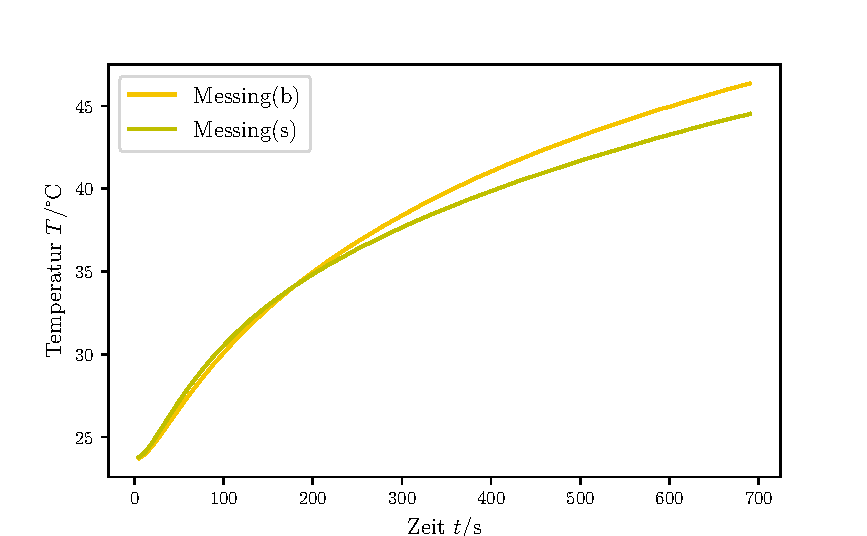
\includegraphics[max width=1.1\linewidth]{plots/plot_t1_t4.pdf}
        \caption{T1, T4.}
        \label{fig:plot_t1_t4}
    \end{subfigure}%
    \begin{subfigure}{.5\textwidth}
        \centering
        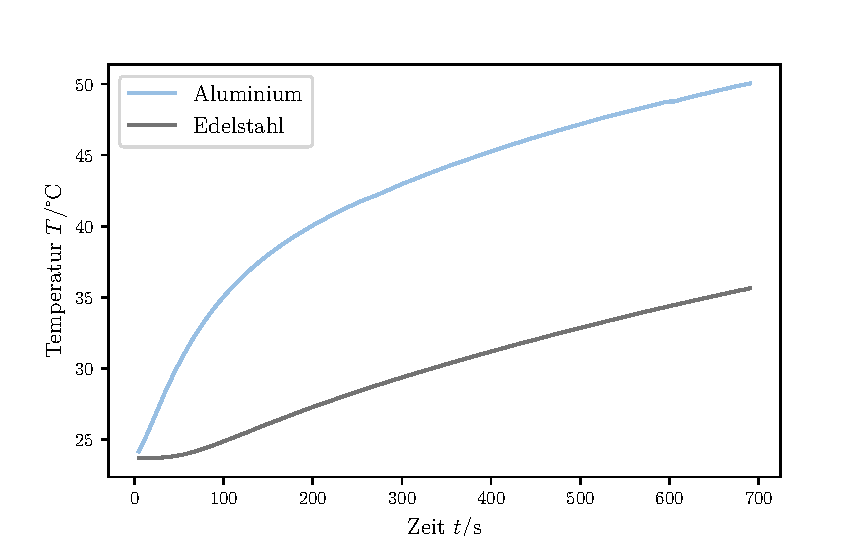
\includegraphics[max width=1.1\linewidth]{plots/plot_t5_t8.pdf}
        \caption{T5, T8}
        \label{fig:plot_t5_t8}
    \end{subfigure}
    \caption{Zeitliche Temperaturverläufe an den äußeren Sensoren}
    \label{fig:tempDiff_t1t4t5t8}
\end{figure}
Sowohl beide Messingproben als auch Aluminium weisen einen ähnlichen Funktionsgraphen auf, der augenscheinlich nur 
in horizontaler und vertikaler Skalierung variiert. 
In den etwa ersten 180 Sekunden steigt die Temperatur des schmalen Messingstabs minimal schneller an als der breite Stab. 
Danach hat der Graph des breiteren Stabs eine größere Steigung und beide Graphen steigen in gleichem Maße, um einen 
stetig wachsenden Temperaturunterschied versetzt, bis zur Endzeit.
Aluminium erreicht insgesamt die höchste Endtemperatur mit etwa $\SI{50}{\celsius}$. 
Im Gegensatz dazu steht Edelstahl: Nach einer kurzen anfänglichen Phase, in der die Temperatur kaum steigt, wächst der 
Graph nahezu linear an, was sich merklich von den Graphen unterscheidet. 
Diese besitzen vielmehr die geschwungene Form einer Wurzel- oder Logarithmus-Funktion. 

Um die Wärmeleitung besser zu untersuchen, sind hier die Endtemperaturen nach annähernd $\SI{700}{\second}$ aufgeführt:
\begin{table}
    \centering
    \caption{Äußere Temperatur nach $\SI{690}{\second}$ in $\SI{}{\celsius}$.}
    \label{tab:temp_aussen}
    \begin{tabular}{S[table-format=3.1, round-mode=places, round-precision=1] S[table-format=2.2] S[table-format=2.2] S[table-format=2.2] S[table-format=2.2]}
        \toprule
        {$t$} & {Messing(b)} & {Messing(s)} & {Aluminium} & {Edelstahl} \\
        \midrule
        690.0 & 46.36 &	44.53 &	50.04 &	35.64  \\
        \bottomrule
    \end{tabular}
\end{table}
Wie bereits erähnt hat Aluminium die höchste Endtemperatur erreicht, danach folgen der breite, der schmale Messingstab 
und Edelstahl in ebendieser Reihenfolge. 
Dementsprechend staffelt sich ebenfalls das zugehörige Maß der Wärmeleitung der einzelnen Proben. 

Nun soll für fünf verschiedene Messzeiten der Wärmestrom bestimmt werden, die sich über die Formel 
\begin{equation}
    \frac{\increment \symup{Q}}{\increment \symup{t}} = -\kappa A \frac{\increment \symup{T}}{\increment \symup{x}}
\end{equation}
berechnen lässt (vgl. dazu die Gleichung \eqref{eqn:waermemenge}). 
Hierbei gelten für Aluminium und Edelstahl ebenso die Maße der breiten Querschnittsfläche 
$\symup{A}_{breit} = \SI{1.2}{\centi\m} \times \SI{0.4}{\centi\m} = \SI{0.48}{\square\centi\m}$,
wohingegen der schmale Messingstab die Maße
$\symup{A}_{schmal} = \SI{0.7}{\centi\m} \times \SI{0.4}{\centi\m} = \SI{0.28}{\square\centi\m}$ 
erfüllt.
Bewusste Messwerte zu fünf verschiedenen Messzeiten und die sich daraus ergebenden Temperaturdifferenzen 
sind in Tabelle \ref{tab:temp_5_messwerte} und \ref{tab:tempdiff_5_messwerte} dargestellt. 
\begin{table}
    \centering
    \caption{Temperatur fünf verschiedener Messzeiten in $\si{\celsius}$.}
    \label{tab:temp_5_messwerte}
    \begin{tabular}{S[table-format=3, round-mode=places, round-precision=1] S[table-format=2.2] S[table-format=2.2] S[table-format=2.2] S[table-format=2.2] S[table-format=2.2] S[table-format=2.2] S[table-format=2.2] S[table-format=2.2]}
        \toprule
        & \multicolumn{2}{c}{Messing(breit)} & \multicolumn{2}{c}{Messing(schmal)} & \multicolumn{2}{c}{Aluminium} & \multicolumn{2}{c}{Edelstahl} \\
        \cmidrule(lr){2-3}\cmidrule(lr){4-5}\cmidrule(lr){6-7}\cmidrule(lr){8-9}
        {$t[\si{\s}]$} & {$T_{1, \text{fern}}$} & {$T_{2, \text{nah}}$} & {$T_{3, \text{nah}}$} & {$T_{4, \text{fern}}$} & {$T_{5, \text{fern}}$} & {$T_{6, \text{nah}}$} & {$T_{7, \text{nah}}$} & {$T_{8, \text{fern}}$} \\
        \midrule
        60  & 27.45 &	31.68 &	32.57 &	27.94 &  31.50 & 34.49 & 29.59 & 24.03 \\
        150 & 32.77 &	36.49 &	36.83 &	32.97 &  38.00 & 40.03 & 34.40 & 26.11 \\
        295 & 38.24 &	41.41 &	40.97 &	37.54 &  42.83 & 44.47 & 38.19 & 29.27 \\
        475 & 42.69 &	45.63 &	44.63 &	41.26 &  46.73 & 48.27 & 41.70 & 32.46 \\
        640 & 45.61 &	48.52 &	47.26 &	43.85 &  49.33 & 50.89 & 44.27 & 34.95 \\
        \bottomrule
    \end{tabular}
\end{table}

\begin{table}
    \centering
    \caption{Temperaturunterschied nah zu fern in $\si{\kelvin}$.}
    \label{tab:tempdiff_5_messwerte}
    \begin{tabular}{S[table-format=3, round-mode=places, round-precision=1] S[table-format=1.2, round-mode=places, round-precision=2] S[table-format=1.2, round-mode=places, round-precision=2] S[table-format=1.2, round-mode=places, round-precision=2] S[table-format=1.2, round-mode=places, round-precision=2]}
        \toprule
        {$t[\si{\s}]$} & {$\increment T_{Messing(breit)}$} & {$\increment T_{Messing(schmal)}$} & {$\increment T_{Aluminium}$} & {$\increment T_{Edelstahl}$} \\
        \midrule
        60  & 4.23   & 4.6299 & 2.99 &	5.559 \\
        150 & 3.7199 & 3.8599 & 2.03 &	8.29 \\
        295 & 3.1699 & 3.4299 & 1.64 &	8.91 \\
        475 & 2.94   & 3.370  & 1.54 &	9.24 \\
        640 & 2.91   & 3.4099 & 1.56 &	9.32 \\
        \bottomrule
    \end{tabular}
\end{table}

Die Werte für die materialabhängige Wärmeleitfähigkeit werden der Tabelle \ref{tab:Literaturwerte} mit den im Vorraus 
recherchierten Literaturwerten entnommen, 
der Abstand zweier Temperatursensoren ist gemäß der Messung $\increment x = \SI{3.0}{\centi\meter}$. 
Daraus ergeben sich die in Tabelle \ref{tab:Warmestrom} dargestellten Zahlenwerte für den Wärmestrom.
\begin{table}
    \centering
    \caption{Wärmestrom $\frac{\increment \symup{Q}}{\increment \symup{t}}$ in $\si{\joule\per\second}$.}
    \label{tab:Warmestrom}
    \begin{tabular}{l | S[round-mode=places, round-precision=4] S[round-mode=places, round-precision=4] S[round-mode=places, round-precision=4] S[round-mode=places, round-precision=4] S[round-mode=places, round-precision=4]}
        \toprule
        {Stoff} & {$\SI{60}{\s}$} & {$\SI{150}{\s}$} & {$\SI{295}{\s}$} & {$\SI{475}{\s}$} & {$\SI{640}{\s}$} \\
        \midrule
        Messing(breit)      & 0.758016    & 0.6666  & 0.56806 & 0.52684   & 0.52147   \\
        Messing(schmal)     & 0.483989  & 0.40349 & 0.358549 & 0.352277 & 0.35645 \\
        Aluminium           & 1.05726    & 0.71780   & 0.57990   & 0.54454   & 0.5516   \\
        Edelstahl           & 0.4092   & 0.61014  & 0.6565119 & 0.68006   & 0.68595   \\
        \bottomrule
    \end{tabular}
\end{table}

Des Weiteren sollen die an den Sensoren T7 und T8 beziehungsweise T2 und T1 gemessenen Temperaturdifferenzen in einem 
Diagramm der Zeit $t$ aufgetragen werden, also die Temperaturunterschiede an zwei verschiedenen Orten desselben Stabs, 
hier Edelstahl und Messing. 
\begin{figure}
    \centering
    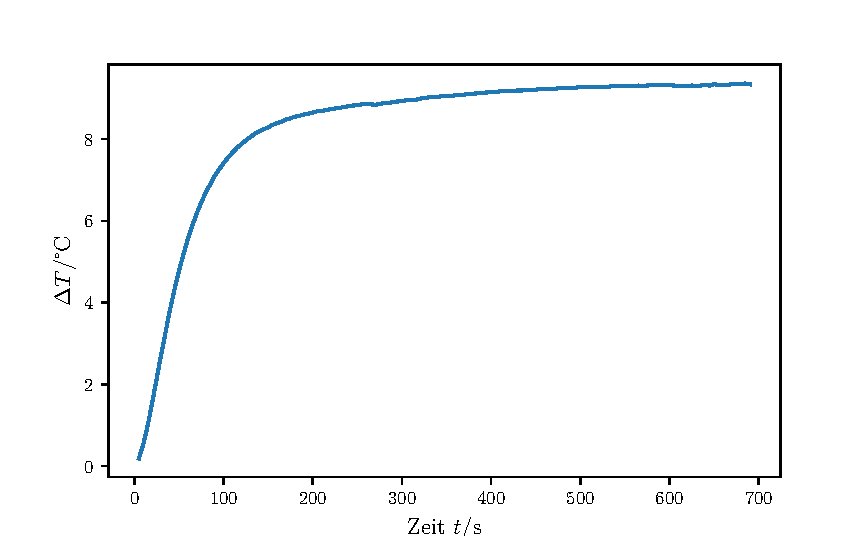
\includegraphics[max width=\linewidth]{plots/plot_tempDiff_steel.pdf}
    \caption{Temperaturdifferenz $T7 - T8$ (Edelstahl).}
    \label{fig:plot_tempDiff_t7t8}
\end{figure}

\begin{figure}
    \centering
    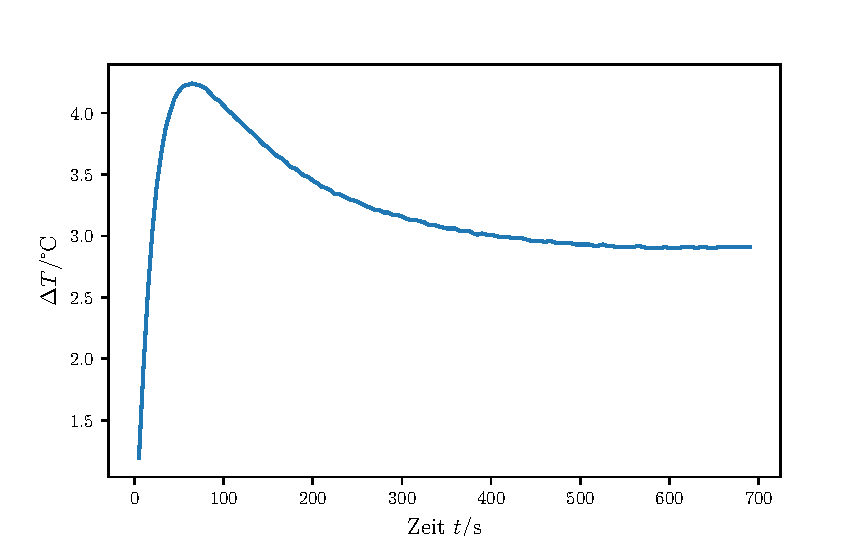
\includegraphics[max width=\linewidth]{plots/plot_tempDiff_brass_wide.pdf}
    \caption{Temperaturdifferenz $T2 - T1$ (Messing).}
    \label{fig:plot_tempDiff_t2t1}
\end{figure}
Beide Graphen haben anfänglich einen starken Anstieg, bei dem Edelstahl einen etwa doppelt so großen Wert erreicht wie Messing. 
Danach flacht die Differenz des Messings exponentiell ab, wohingegen die des Edelstahls sich asymptotisch einem Maximalwert nähert. 
Das zu Beginn starke Ansteigen indiziert das Anlegen einer dem Metall gegenüber höheren Temperatur, die zuerst am nahen 
Sensor registriert wird und erst mit einiger Zeitverzögerung an der weiter entfernten Messstelle. 
Die Temperaturdifferenz des Edelstahls steigt weiter an, das Temperaturgefälle nimmt also zu.
Dahingegen findet beim Messing ein schleichender Ausgleich der hohen Differenz statt, die Wärme verteilt sich gleichmäßiger auf dem Stab.  

\begin{table}
    \centering
    \caption{Messreihe 2 - Dynamische Methode}
    \label{tab:data2}
    \begin{tabular}{S[table-format=3.1, round-mode=places, round-precision=1] S[table-format=2.2] S[table-format=2.2] S[table-format=2.2] S[table-format=2.2] S[table-format=2.2] S[table-format=2.2] S[table-format=2.2] S[table-format=2.2]}
        \toprule
        & \multicolumn{2}{c}{Messing(breit)} & \multicolumn{2}{c}{Messing(schmal)} & \multicolumn{2}{c}{Aluminium} & \multicolumn{2}{c}{Edelstahl} \\
        \cmidrule(lr){2-3}\cmidrule(lr){4-5}\cmidrule(lr){6-7}\cmidrule(lr){8-9}
        {$t$} & {$T_{1, \text{fern}}$} & {$T_{2, \text{nah}}$} & {$T_{3, \text{nah}}$} & {$T_{4, \text{fern}}$} & {$T_{5, \text{fern}}$} & {$T_{6, \text{nah}}$} & {$T_{7, \text{nah}}$} & {$T_{8, \text{fern}}$} \\
        \midrule
        0.000 & 33.08 &	36.21 &	36.46 &	32.47 &	34.62 &	37.16 &	33.62 &	29.54 \\
        0.500 & 33.10 &	36.25 &	36.48 &	32.50 &	34.66 &	37.19 &	33.65 &	29.55 \\
        1.000 & 33.12 &	36.27 &	36.51 &	32.52 &	34.69 &	37.25 &	33.68 &	29.54 \\
        $\vdots$ & $\vdots$ & $\vdots$ & $\vdots$ & $\vdots$ & $\vdots$ & $\vdots$ & $\vdots$ & $\vdots$ \\
        882.00 & 65.16 & 65.67 & 62.65 & 61.61 & 67.34 & 65.75 & 62.62 & 50.17 \\
        \bottomrule
    \end{tabular}
\end{table}